\sloppy
\section{Perception Lab: The Experiments Behind the Engine}
\label{app:lab}

This appendix records the nine perception experiments from which the engine of Section~\ref{sec:perception} was taken. Each experiment is a single Python file that takes one screenshot of a game frame and returns an image and a short text for a model to read. The code and all outputs are released with the paper (Appendix~\ref{app:reproduce}).

\subsection{Setup}
\label{sec:lab}

\paragraph{Shared front end.}
All eight new experiments (X1--X8) share one front end, so that only the presentation changes. A screenshot is turned into an exact $64{\times}64$ palette-index grid (the cell pitch and origin are fitted from colour edges, and each cell takes the nearest palette colour). The grid is split into terrain (large colour fields), 4-connected objects with a kind (object, icon, dotted figure, thin line or bar), special boxes (panels) and status items at the screen edge (HUD). Every experiment then computes something on top of these objects.

\paragraph{Baseline.}
The baseline is our first perception module, the \emph{Legacy Encoder} (\code{arc\_eye}). It also works from a screenshot and prints a text report only, so the model never sees pixels: the fitted lattice, a palette-stable symbol per cell, terrain versus objects, connected components with holes, symmetry and a dihedral shape hash, composite objects, dotted chains and bars, and a diff with object tracking against the previous frame. It costs about 3{,}500 text tokens per frame.

\paragraph{Test frames and grading.}
The two test frames are the first levels of \code{ls20} (keyboard controls) and \code{r11l} (clicks). Before any experiment ran, we wrote an answer key of seven items per game and checked it against the game engine: K1 what is controlled, K2 the goal, K3 the link or body (for \code{ls20}, the inventory icon and the lock glyph; for \code{r11l}, the disc that sits at the midpoint of its two handles), K4 the modifier or hazard, K5 the status items, K6 a winning plan, and K7 the terrain. For each item, an output scored 2 if it stated or showed the item correctly and unmistakably, 1 if only partly, 0 if absent and $-1$ if it stated something that would mislead; the maximum is 14 per game and 28 in all. We also gave an intuition grade from 1 to 5 (how quickly a player reading only this output would understand the game) and recorded the text cost. The grader was the same agent that built the experiments and it knew both games, so it graded only what each output itself states. No blind reader was used.

\subsection{The Experiments}
\label{sec:lab-exps}

\begin{description}
    \item[X1 Exploded Inventory.] Objects are de-duplicated by their exact colour grid. Each kind is pulled out of the scene, enlarged to a common readable size (the bounding-box cells that are empty are drawn as a checker so that holes read as holes), spaced apart, labelled with a letter, and marked $\times N$ when it has $N$ copies. A small thumbnail of the frame outlines where each one sits, and the legend gives its zone, its ground colour and its coordinates. Thin lines are listed with their end points. The motivation is that vision-language models fail on small, close shapes but succeed when the shapes are separated \citep{rahmanzadehgervi2024blind}.
    \item[X2 Surprise Map.] The surprise of a cell is $-\log_2 p$, where $p$ is the frequency of its $3{\times}3$ neighbourhood pattern in this frame. Repeated texture (floor, walls, tiles) scores near zero bits, and a pattern seen at least eight times counts as predictable. Objects are ranked by the total bits of their cells, the top eight keep full colour on an otherwise faded frame, and a symmetry-break test flags an object whose \emph{shape} is symmetric under a mirror or quarter turn while its \emph{colouring} is not, reporting the side that holds the odd colour.
    \item[X3 Visual Routines.] Four serial routines in the sense of \citet{ullman1984visual}, run in code. \textbf{Reach} picks the most self-like object (not at the screen edge, at least two colours, at least nine cells, square first). If the game has a tile of side $u$, it flood-fills the floor in steps of $u$ and reports the step count to every object, or the side of a box where the floor ends. Without a tile grid it takes the open-space fraction and sweeps the smaller object's footprint along the straight line between each pair, counting rock cells hit. \textbf{Fit} lists which objects sit inside which box and which hollow figures enclose an empty space, giving its size and the objects that fit it exactly. \textbf{Trace} follows each thin line from its two end points (cells with at most one neighbour) to the nearest objects, and reports an object linked to exactly two others that lies within one cell of their midpoint. \textbf{Align} reports pairs that share at least 60\% of their columns or rows.
    \item[X4 Look-alike Threads.] For every pair of objects, the binary shapes are compared under the eight rotations and flips and under integer scale factors 1, 2 and 3. The relation is \textsc{exact} (a copy, which also marks counters), \textsc{turned} (equal after a rotation, flip or rescale, with the transform named), \textsc{near} (equal size, a few cells differ, and how many), or \textsc{state} (same shape, different colour). A colour shared by three or more different things is reported as a colour link. Threads joining matched objects are drawn on the frame.
    \item[X5 Foresight Strip.] The next frame is imagined for every action from four priors: an agent moves by its own size along the floor and stops at walls; the longest HUD bar is a budget that drops one unit per action; of two same-shaped objects the brighter is selected, and clicking empty space sends it there; and an object held at the midpoint of two anchors stays at their midpoint. For click games it searches symmetric anchor placements for the cheapest collision-free three-click plan. The game engine is used only afterwards to score the predictions, in a file the reader never sees.
    \item[X6 Blueprint.] The frame is redrawn as a schematic after \citet{marr1982vision}: floor in beige, walls and void hatched, the tile lattice drawn faintly, special boxes outlined in yellow, every object outlined and lettered with a shape word, and the HUD moved out of the map into a labelled side panel, with gauges described by their length.
    \item[X7 Role Ledger.] Each object is scored against nine roles (\textsc{you}, \textsc{goal}, \textsc{modifier}, \textsc{inventory}, \textsc{moves left}, \textsc{lives}, \textsc{handle}, \textsc{carried thing}, \textsc{scenery}) with hand-set evidence points from design priors and from the outputs of X2--X4. A long bar at the edge adds to \textsc{moves left}; identical copies at the edge add to \textsc{lives}; the most self-like object adds to \textsc{you} (more if its size equals the floor tile); a hollow outline whose inside fits another object adds to \textsc{goal}; a HUD icon that matches a world object adds to \textsc{inventory} and \textsc{goal}. A role's probability is its score divided by the object's total score plus one. Every top hypothesis is printed with its evidence and the cheapest action that would confirm or kill it.
    \item[X8 Fused Briefing.] Built after X1--X7 were graded and after the held-out check of Section~\ref{sec:holdout}. It uses the Blueprint canvas as its picture, draws the dashed threads of X4 and the midpoint ring of X3 on it, and writes two tiers of text: \textsc{measured} (the facts of X3, X4 and the symmetry-break test of X2) and \textsc{guesses} (the roles of X7 with their confidence and one-action test). Objects carry the same letters in picture and text. X5 was dropped because its priors failed out of sample, and X1 and X2 on their own added too little.
\end{description}

\subsection{Results on the Two Test Frames}
\label{sec:lab-results}

\begin{table}[t]
\centering
\small
\setlength{\tabcolsep}{3pt}
\begin{tabular}{@{}L{0.37\columnwidth}rrrrr@{}}
\toprule
Presentation & \code{ls20} & \code{r11l} & Total & Int. & Tokens \\
 & /14 & /14 & /28 & 1--5 & \\
\midrule
Legacy Encoder (baseline) & 2 & 1 & 3 & 1 & 3500 \\
X1 Exploded Inventory & 2 & 1 & 3 & 2 & 180 \\
X2 Surprise Map & 3 & 1 & 4 & 2 & 270 \\
X3 Visual Routines & 7 & 8 & 15 & 4 & 240 \\
X4 Look-alike Threads & 4 & 2 & 6 & 3 & 140 \\
X5 Foresight Strip & 4 & 8 & 12 & 4 & 140 \\
X6 Blueprint & 4 & 4 & 8 & 3 & 100 \\
X7 Role Ledger & 11 & 9 & 20 & 5 & 380 \\
X8 Fused Briefing & 13 & 12 & 25 & 5 & 370 \\
\bottomrule
\end{tabular}
\caption{Rubric score per game, intuition grade (Int.) and text tokens per frame. The Legacy Encoder also marked the move counter of \code{r11l} as screen chrome ($-1$). X8 was designed after the others were graded and was graded on the same two frames.}
\label{tab:lab}
\end{table}

\begin{figure*}[t]
\centering
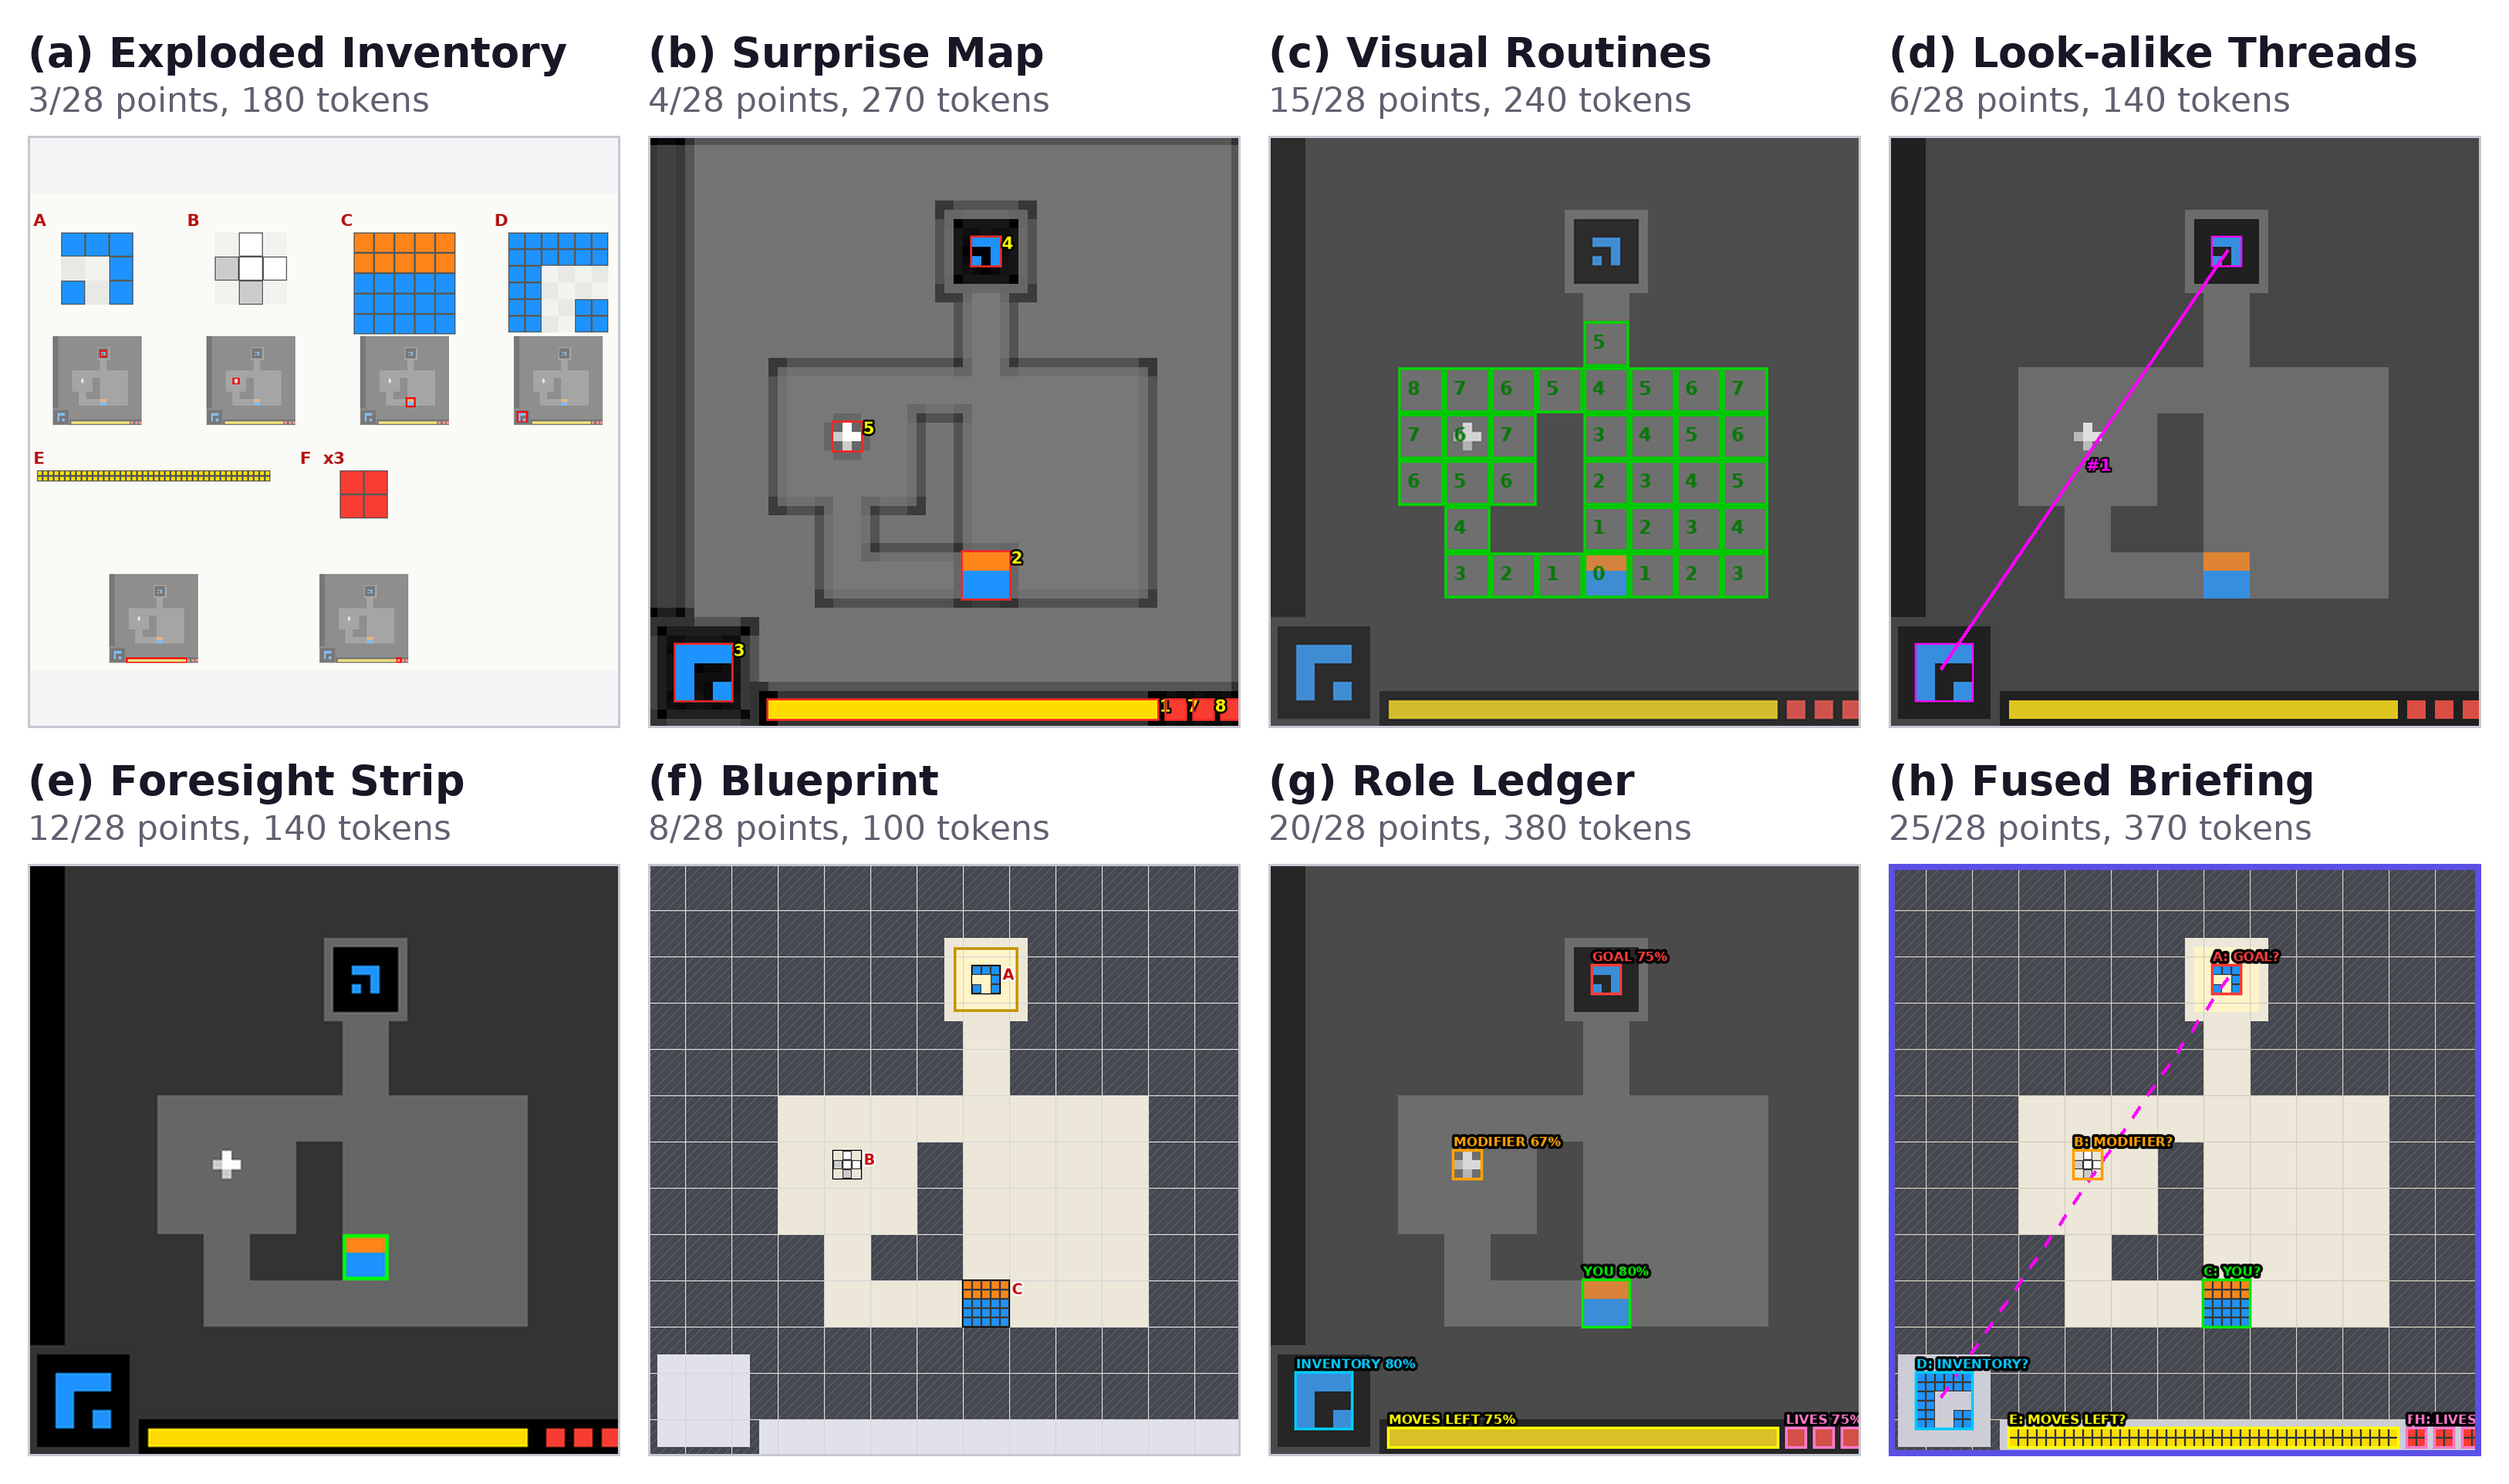
\includegraphics[width=\textwidth]{figures/png/perception_lab_gallery.png}
\caption{The image part of each candidate presentation for the opening frame of \code{ls20}, with its rubric score and its text cost per frame. (a) Exploded Inventory pulls out every object and stacks copies. (b) Surprise Map keeps colour only where the frame is unpredictable. (c) Visual Routines marks reachability, with the step count to each tile. (d) Look-alike Threads joins shapes that match under rotation, mirroring or scale. (e) Foresight Strip imagines the next frame (here, one step up). (f) Blueprint redraws floor, walls and lattice as a clean schematic. (g) Role Ledger tags each object with a guessed role and a confidence. (h) Fused Briefing, the presentation we kept, combines the blueprint with measured facts and tagged guesses.}
\label{fig:labgallery}
\end{figure*}

\begin{figure}[t]
\centering
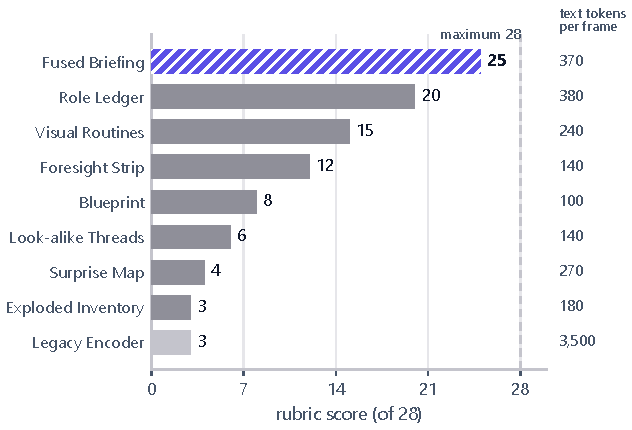
\includegraphics[width=\columnwidth]{figures/perception_lab.pdf}
\caption{Rubric score (of 28) and text tokens per frame for the Legacy Encoder and the eight presentations, on the two test frames. The Fused Briefing scores 25/28 against 3/28 for the Legacy Encoder at about a tenth of the text.}
\label{fig:lab}
\end{figure}


Table~\ref{tab:lab} and Figure~\ref{fig:lab} give the scores and Figure~\ref{fig:labgallery} shows the image part of each presentation. Three things moved understanding. The \emph{computed relations} of X3 and X4 state facts that a model cannot reliably read off a picture: on \code{r11l} X3 found the midpoint tether and the ring that fits a $5{\times}5$ object, and on \code{ls20} X4 showed that the inventory icon is the lock glyph turned $90^\circ$ and drawn at twice the size. The \emph{role labels} of X7 gave the fastest gist, with every role right on both frames. The \emph{foresight} of X5 predicted all four \code{ls20} moves and the gauge, and its three-click plan solved \code{r11l}. X1 and X2 were no better than the Legacy Encoder, and X6 is the best map for navigation but says nothing about meaning. The Fused Briefing scored 25/28 at about 370 tokens per frame, $8.3\times$ the Legacy Encoder's score with 89.4\% fewer text tokens. Because the grader knew both games and X8 was graded on the frames it was designed on, these scores are optimistic.

\subsection{Held-Out Check: Facts Versus Guesses}
\label{sec:holdout}

We then checked X5 and X7 on the 23 other official games, none of which was used in the design. The checker synthesises a screenshot from each game's reset frame ($7$ pixels per cell) and sends it through the normal loader, and ground truth comes from the game engine only: the agent is the objects whose cells change under the arrow actions, an object responds to clicks if clicking its centre changes any non-HUD cell, and the gauge is right if the bar the ledger calls \textsc{moves left} changes after one action (Table~\ref{tab:holdout}). Turning a screenshot into a grid generalised perfectly. The guesses did not: they had effectively been fitted to the two test frames, and were right about half the time or less on unseen games.

\begin{table}[t]
\centering
\small
\begin{tabular}{@{}L{0.55\columnwidth}L{0.36\columnwidth}@{}}
\toprule
Check on the 23 held-out games & Result \\
\midrule
Screenshot to grid, exact cells & 23/23 games \\
Agent identity (X7), keyboard games & 6/14 games \\
Moves-left gauge found (X7) & 10/20 games \\
Click handles that respond (X7) & 7/29 handles \\
Keyboard foresight fully right (X5) & 1/16 games \\
\bottomrule
\end{tabular}
\caption{Held-out check of the single-frame guesses. For click handles, the guesses were good on \code{dc22} (2/2), \code{sb26} (4/4) and \code{ka59} (1/1) and bad on \code{lp85} (0/17). On two further keyboard games nothing moved on the first key press, so the agent-identity guess could not be checked.}
\label{tab:holdout}
\end{table}

This fixed the design rule of the engine: measured relations (X3, X4) are true by construction and carry no such risk, so they are stated as facts, whereas roles and dynamics from one frame are stated as guesses with a one-action test. We did not run the Fused Briefing as a whole on the held-out games, and the lab reports no RHAE. The end-to-end effect of the engine on the agent is not isolated by an ablation: the trajectory of Section~\ref{sec:trajectory} changes several components at once.

\section{Perception Engine Structural Briefings}
\label{app:briefings}

Below we provide the verbatim structured briefing text emitted by the deterministic perception engine for the opening frames of \code{ls20} and \code{r11l} illustrated in Figure~\ref{fig:views}. The object identifiers correspond exactly with the annotated spatial map and the kernel's symbolic state dictionary (\code{observe().objects}).

\paragraph{\code{ls20} Opening Frame (Discrete Navigation Grid):}
\begin{lstlisting}
BRIEFING (arrow keys)
MEASURED (certain):
- Floor is a 5x5 tile grid.
- obj 4 (blue 6-cell shape): sits inside a black box that is NOT plain floor; the floor reaches the box's bottom side in 5 steps (the only way in)
- obj 6 (white/light grey plus): reachable in 6 steps
- obj 4 (blue 6-cell shape) is directly above obj 10 (blue/orange square) (shared columns 35-37)
- obj 12 (blue irregular shape (24 cells)) (drawn 2x bigger), mirrored left-right OR turned 90 deg clockwise, becomes exactly obj 4 (blue 6-cell shape)
- 3 identical red square (2x2): obj 16, 17, 18 -> a count of something (lives, items, tiles)
- obj 6 (white/light grey plus) has a symmetric shape but lopsided colours (marks a direction/state)
- obj 10 (blue/orange square) has a symmetric shape but lopsided colours (marks a direction/state)
GUESSES (check with one action):
- obj 10 (blue/orange square) = YOU (80%) - test: press one arrow key: it should move one tile and the gauge should drop
- obj 12 (blue irregular shape (24 cells)) = INVENTORY (80%) - test: watch it after touching the modifier
- obj 4 (blue 6-cell shape) = GOAL (75%) - test: get the right thing into it and see if the level ends
- obj 15 (yellow bar) = MOVES LEFT (75%) - test: take any action and check it shrinks by one unit
- obj 16, 17, 18 (red square) = LIVES (75%) - test: watch it when the gauge runs out or you fail
- obj 6 (white/light grey plus) = MODIFIER (67%) - test: step onto it, then check whether the inventory icon changed
\end{lstlisting}

\paragraph{\code{r11l} Opening Frame (Continuous Coordinate Space):}
\begin{lstlisting}
BRIEFING (clicks)
MEASURED (certain):
- no tile grid -> free movement. Open space = black (81% of screen).
- all 4 main objects share one open space; straight paths between them are ALL CLEAR of rock
- the grey areas are not open floor (likely walls)
- obj 4 (purple dotted ring) encloses an EMPTY 5x5 space -- exactly the size of: obj 16 (white/purple diamond), obj 25 (purple/magenta disc), obj 36 (dark grey/purple diamond)
- a light grey line connects obj 16 (white/purple diamond) to obj 25 (purple/magenta disc)
- a light grey line connects obj 25 (purple/magenta disc) to obj 36 (dark grey/purple diamond)
- obj 25 (purple/magenta disc) sits at the MIDPOINT of obj 16 (white/purple diamond) and obj 36 (dark grey/purple diamond) (error 0.5 cells) -> it is held between them; moving either end should move it to the new midpoint
- obj 16, 36 (white/purple diamond; dark grey/purple diamond) have the same shape in different colours (white/purple vs dark grey/purple)
GUESSES (check with one action):
- obj 4 (purple dotted ring) = GOAL (80%) - test: get the right thing into it and see if the level ends
- obj 16, 36 (white/purple diamond; dark grey/purple diamond) = HANDLE (click) (80%) - test: click an empty spot once: the selected handle should jump there
- obj 1 (white bar) = MOVES LEFT (75%) - test: take any action and check it shrinks by one unit
- obj 25 (purple/magenta disc) = CARRIED THING (75%) - test: move one handle: it should slide to the new midpoint
\end{lstlisting}

\section{System Configuration and Hyperparameters}
\label{app:config}

Table~\ref{tab:hyperparams} documents the primary execution parameters governing the scored benchmark evaluation.

\begin{table}[h]
\centering
\footnotesize
\setlength{\tabcolsep}{4pt}
\begin{tabular}{@{}L{0.52\columnwidth}L{0.44\columnwidth}@{}}
\toprule
System Configuration Parameter & Operational Value \\
\midrule
Concurrent games / Active GPU slots & 25 games / 10 slots \\
Scheduler quantum allocation & 20 model calls per round \\
Action allocation ceiling per game & 2,000 actions \\
Maximal steps per \code{play()} path & $\le$100 actions \\
Turn reply budget / Inner requests & 12k tokens / 12 calls \\
Turn preemption thinking threshold & 16k tokens \\
Context drain threshold / target & 118k tokens / 55k tokens \\
Context maximum window size & 131,072 tokens \\
Visual map rendering scale & 10 pixels per grid cell \\
Briefing line limit / Short-view ceiling & 20 lines / 600 tokens \\
Symbolic memory caps (\code{G}/\code{P}/\code{H}/\code{F}) & 150 / 200 / 400 / 300 tokens \\
Sampling temperature / top-$p$ / top-$k$ & $T = 0.6$ / $p = 0.95$ / $k = 20$ \\
Serving engine and precision & SGLang, W4A16, FP8 KV cache \\
Speculative decoding configuration & EAGLE (3 speculative draft steps) \\
\bottomrule
\end{tabular}
\caption{System hyperparameter settings deployed in the official evaluation runtime.}
\label{tab:hyperparams}
\end{table}

\section{Artifacts and Reproducibility}
\label{app:reproduce}
All empirical findings, telemetry traces, and figures in this manuscript are fully reproducible using the scripts in \code{Writing/scripts/}:
\begin{itemize}
    \item \code{collect\_data.py}: Ingests the Kaggle submission log, per-game benchmark tables, and perception lab evaluation rubrics.
    \item \code{extract\_curves.py}: Extracts wall-clock level completion trajectories from raw execution logs.
    \item \code{make\_perception\_figure.py}: Executes the host-side perception engine on raw game environments to generate segmented objects, spatial maps, and structured briefings.
    \item \code{plot\_results.py}: Generates all publication-grade figures in vector PDF and high-resolution raster formats.
\end{itemize}
All code, model serving scripts, evaluation environments, and experimental logs are publicly accessible under the MIT-0 license (a permissive public-domain-equivalent license, as the competition rules require) at \url{https://github.com/Harsidak/SARBLOH}.